\begin{Q}
\textbf{\Large K-Means 1}\\

\begin{enumerate}

\item Mention if K-Means is a supervised or an un-supervised method and state the reason.

\item Assume that you are trying to cluster data points $x_{i}$  for $ i \in \{1,2, \dots, D\}$ into $K$ clusters each with center $\mu_{k}$  where $ k \in \{1,2, \dots, K \}$. The objective function for doing this clustering involves minimization of the Euclidean distance between the points and the cluster centers. It is given by  \begin{equation*}
\min\limits_{\mu} \min\limits_{r}\sum\limits_{i \in D} \sum\limits_{k =1}^{K} \frac{1}{2} r_{ik} \|x_{i} -\mu_{k}\|_{2}^{2}. \\
 \end{equation*} \\ How do you ensure hard assignment of one data point to one and only one cluster at a given time?
 
 \textbf{Hint:} By hard assignment we mean that you are 100 \% sure that a point either belongs or doesn't belong to a cluster.
 
 \item How does your answer to part b change if we want to obtain a soft assignment instead?
 
 \textbf{Hint:} By soft assignment we mean that  a point  belongs to a cluster with some probability.
 
 \item Looking at the following plot, what is the best choice for the number of clusters?
 \begin{center}
 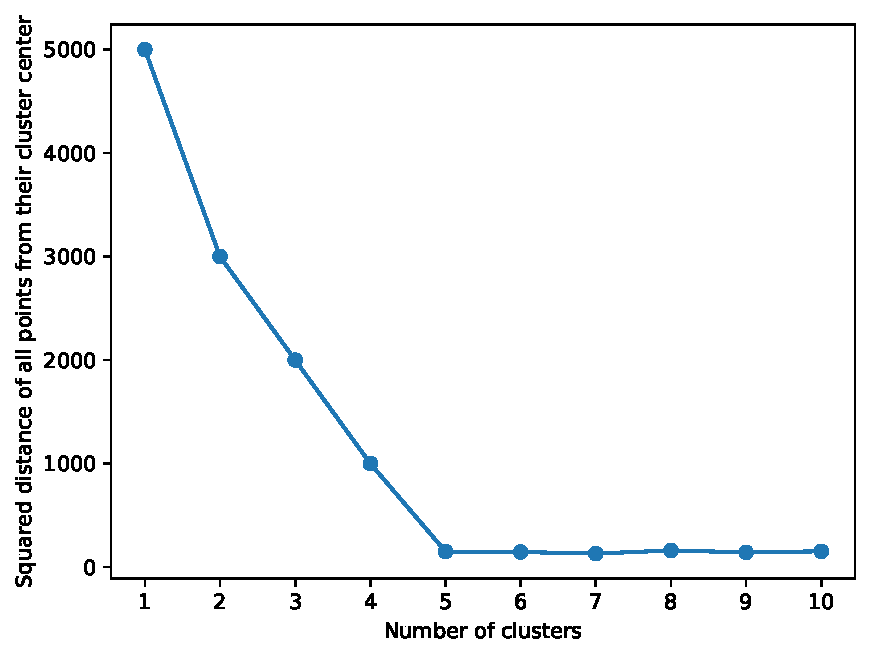
\includegraphics[width=8cm]{figs/cluster.pdf}
 \end{center}
 
 \item Would K-Means be an efficient algorithm to cluster the following data? Explain your answer in a couple of lines.
 \begin{center}
 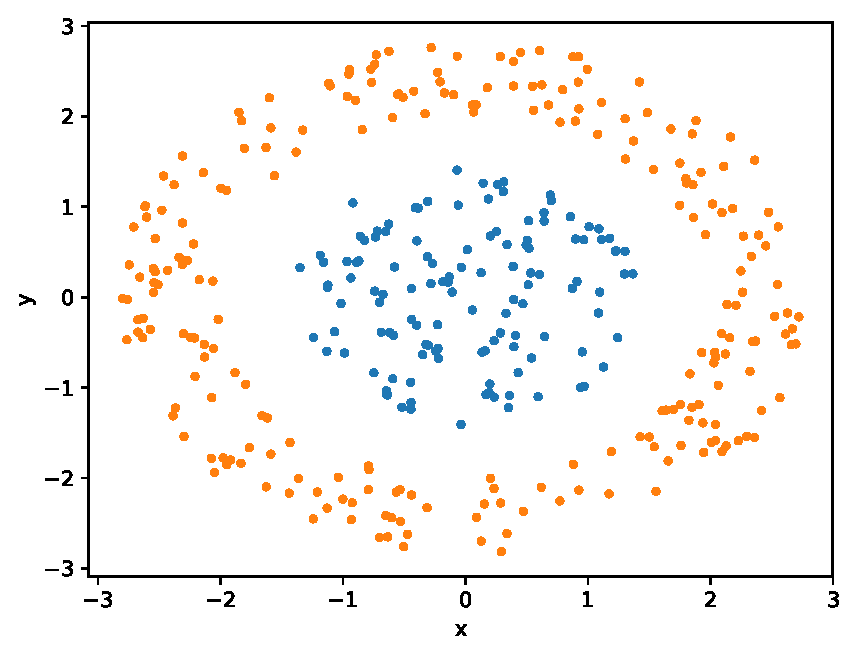
\includegraphics[width=8cm]{figs/concentric.pdf}
 \end{center}

\end{enumerate}


\end{Q}
          